\documentclass[11pt]{beamer}

\mode<presentation>
\usetheme{Copenhagen}
\setbeamertemplate{navigation symbols}{} 
\setbeamertemplate{caption}[numbered]
\setbeamercolor{block title}{bg=blue}

\usepackage[utf8]{inputenc}
\usepackage{amsmath}
\usepackage{amsfonts}
\usepackage{amssymb}
\usepackage{gensymb}
\usepackage{tikz}

\usetikzlibrary{arrows.meta}

%\author{Alexey L. Cherezov}
\title{Fuel Rod Analysis Program Interface \\(FRAPI)}
%\setbeamercovered{transparent} 
%\setbeamertemplate{navigation symbols}{} 
%\logo{} 
\institute{UNIST Core} 
%\date{} 
%\subject{} 

\definecolor{applegreen}{rgb}{0.2, 0.71, 0.0}
\definecolor{bittersweet}{rgb}{1.0, 0.44, 0.37}

\tikzset{%
  >={Latex[width=2mm,length=2mm]},
            base/.style = {rectangle, rounded corners, draw=black,
                           minimum width=4cm, minimum height=1cm,
                           text centered, font=\sffamily},
  box0/.style = {base, minimum width=2.5cm, fill=white!15, align=center},
  box1/.style = {base, minimum width=2.5cm, fill=blue!15, align=center},
  box2/.style = {base, minimum width=2.5cm, fill=red!5, align=center},  
  box3/.style = {base, minimum width=2.5cm, fill=green!15, align=center},    
  void/.style = {base, minimum width=2.5cm, fill=white!30, draw=white, align=left},
}


\begin{document}

\titlepage
\begin{frame}{Outlines:}
    \normalsize
%    \tableofcontents
    \center
    \begin{itemize}
        \item FRAPI Structure and Capability 
        \item FRAPI Usage Example
        \item IFA-432 Benchmark for FRAPCON cross-verification
        \item CABRI REP-NA Benchmark for FRAPTRAN cross-verification
        \item Single Rod RIA Analysis with the Time Step Control
    \end{itemize}
\end{frame}
\begin{frame}{}
    \centering
    \Huge{FRAPI}\\
    \Huge{Structure and Capability}
\end{frame}
\begin{frame}{FRAPI Abilities}

    \centering{\textbf{FRAPI Features:}}

  \begin{block}{}
  1. Provides an access to the most of variables and subroutines of FRAPCON and FRAPTRAN.
  \textit{\small Except of the decay model ANS-5.1 and the fission gas model ANS-5.4}
  \end{block}

  \begin{block}{}
  2. Exchanges the fuel rod data with an external code ``on the flight", at every time step
  \end{block}

  \begin{block}{}
  3. Dumps the fuel rod data in output file for future restart of the calculation, starting of any chosen time moment
  \end{block}
  
\end{frame}
\begin{frame}{RAST-K Burnup and Transient Loops}

  \scriptsize

  \begin{figure}[h]
    \includegraphics[width=0.9\textwidth]{figs/coupling_loops}
  \end{figure}  

\end{frame}
\begin{frame}{Multiphysics Module}

    \scriptsize

    \begin{block}{Interface functions}
        \begin{itemize}
            \item INIT: reading of input data and initialization
            \item SET/GET: allow the access to the fuel rod variables
            \item NEXT: run the new time step
            \item LOAD/SAVE: load and save of the fuel rod state
            \item FINALIZE: clean memory
        \end{itemize}
    \end{block}

    \begin{block}{}
        FRAPI provides the interface functions for a single fuel rod, while
        the Multiphysics module provides for all fuel rods in the lattice
    \end{block}

  \begin{figure}[h]
    \includegraphics[width=0.8\textwidth]{figs/multiphysics_module}
  \end{figure}  

\end{frame}
\begin{frame}{FRAPI Memory Structure}

  \scriptsize

  \begin{figure}[h]
    \includegraphics[width=0.8\textwidth]{figs/frapi_memory_structure}
  \end{figure}  

\end{frame}
\begin{frame}{FRAPI Memory Spaces}

  \scriptsize

    \begin{block}{Memory Spaces (MS)}
        \begin{itemize}
            \item KERNEL: where FRAPTRAN/FRAPCON does calculations
            \item WORKING: stores the current fuel rod state
            \item BACKUP: stores any previous fuel rod state (for restart)
        \end{itemize}
    \end{block}

  \begin{figure}[h]
    \includegraphics[width=0.9\textwidth]{figs/memory_communications}
  \end{figure}  

\end{frame}
\begin{frame}{FRAPI Designation}

    \centering{\textbf{The new program interface for FRAPCON and FRAPTRAN}}

 \begin{center}
 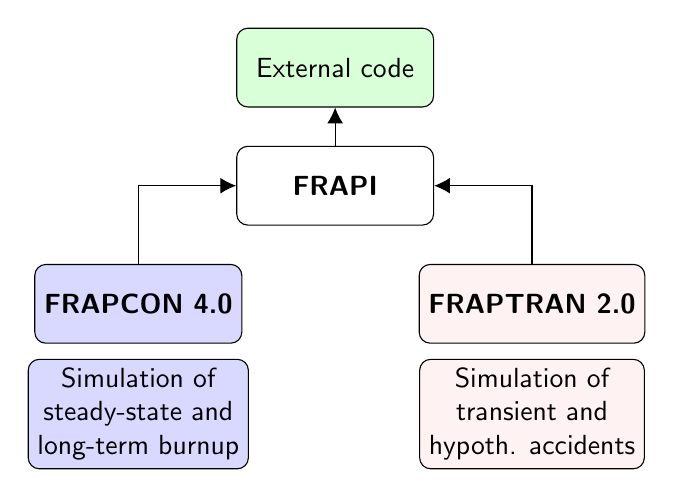
\begin{tikzpicture}[node distance=1.5cm, align=center]

  \node (onFRAPI)    [box0]                                   {\textbf{FRAPI}};
  \node (onCode)     [box3, above of=onFRAPI               ]  {External code};
  \node (onFRAPCON)  [box1, below of=onFRAPI, xshift=-2.5cm]  {\textbf{FRAPCON 4.0}};
  \node (onFRAPTRAN) [box2, below of=onFRAPI, xshift= 2.5cm]  {\textbf{FRAPTRAN 2.0}};  
  \node (on_text_1)  [box1, below of=onFRAPCON, yshift=0.1cm, xshift=0.cm]  {Simulation of \\ steady-state and \\ long-term burnup};
  \node (on_text_2 ) [box2, below of=onFRAPTRAN, yshift=0.1cm, xshift=0cm]  {Simulation of \\ transient and \\ hypoth. accidents};  

  \draw[<-]      (onFRAPI) -| (onFRAPCON);
  \draw[<-]      (onFRAPI) -| (onFRAPTRAN);
  \draw[->]      (onFRAPI) -- (onCode);  
  \end{tikzpicture}
  \end{center} 

\end{frame}
\begin{frame}{FRAPTRAN 2.0 Flowchart}

  \scriptsize

  \begin{figure}[h]
    \includegraphics[width=0.8\textwidth]{figs/fraptran_flowchart}
  \end{figure}  

\end{frame}
\begin{frame}{}
    \centering
    \Huge{FRAPI Usage Example}\\
\end{frame}


\begin{frame}{FRAPI Usage Example Scheme}
  \footnotesize
  \texttt{
  \begin{columns}
  \column{0.48\textwidth}
  \begin{block}{}
    {\color{magenta}PROGRAM} MAIN\\
    {\color{magenta}USE} frapi, {\color{magenta}ONLY}: frodtype\\
    {\color{magenta}TYPE} (frodtype) FR\\    
    {\color{gray}!--- Setup mesh size -----}\\
    {\color{magenta}CALL} FR $\%$ MAKE(<arguments>)\\
    {\color{gray}!--- Setup initial state ----}\\    
    {\color{magenta}CALL} FR $\%$ SET({\color{orange}"name"}, var)\\
    {\color{magenta}CALL} FR $\%$ INIT \\
    {\color{magenta}CALL} FR $\%$ GET({\color{orange}"name"}, var)\\
  \end{block}
  \column{0.48\textwidth}
  \begin{block}{}
    {\color{gray}!--- Burnup/Transient loop --}\\        
    {\color{magenta}DO} i = 1, N\\
    {\color{gray}!--- Trial time step --------}\\            
    {\hspace{5mm}\color{magenta}CALL} FR $\%$ SAVE{\color{gray} ! optional}\\
    {\hspace{5mm}\color{magenta}CALL} FR $\%$ SET({\color{orange}"name"}, var)\\
    {\hspace{5mm}\color{magenta}CALL} FR $\%$ NEXT(dtime)\\
    {\hspace{5mm}\color{magenta}CALL} FR $\%$ GET({\color{orange}"name"}, var)\\
    {\hspace{5mm}\color{magenta}CALL} FR $\%$ LOAD{\color{gray} ! optional}\\
    {\color{magenta}ENDDO} \\
    {\color{gray}!--- Finilize ---------------}\\                    
    {\color{magenta}CALL} FR $\%$ DESTROY()\\            
    {\color{magenta}END PROGRAM}  MAIN
  \end{block}
  \end{columns}
  }
\end{frame}

\begin{frame}{Minimal Example}

    \footnotesize
    \texttt{frapi/debugtests/test2}

  \begin{figure}[h]
    \includegraphics[width=1.0\textwidth]{figs/test_1}
  \end{figure}  

\end{frame}


\begin{frame}{Minimal Example (continuous)}

  \begin{figure}[h]
    \includegraphics[width=1.0\textwidth]{figs/test_2}
  \end{figure}  

\end{frame}


\begin{frame}{Minimal Example (continuous)}

  \begin{figure}[h]
    \includegraphics[width=1.0\textwidth]{figs/test_3}
  \end{figure}  

\end{frame}


\begin{frame}{List of ''\texttt{make}`` arguments}
  
  \footnotesize

  \begin{block}{}
    \begin{enumerate}
    \item \texttt{nr}       : number of radial segments in a pellet (default 17)
    \item \texttt{nce}      : number of radial segments in a cladding (default 10)
    \item \texttt{na}       : number of axial segments (default 10)
    \item \texttt{ngasr}    : number of radial segments for gas release model (default 45)
    \item \texttt{frapmode} : 'frapcon' or 'fraptran' mode
    \item \texttt{mechan}   : 'FEA' or 'FRACAS-I' mechanical model
    \item \texttt{ngasmod}  : fission gas release model
    \item \texttt{icm}      : cladding type (default Zircaloy-4)
    \item \texttt{icor}     : crud model (none, constant or time dependent)
    \item \texttt{iplant}   : PWR, BWR or HBWR plant type
    \item \texttt{imox}     : MOX or UOX fuel type
    \end{enumerate}
  \end{block}

\end{frame}


\begin{frame}{List of ''\texttt{make}`` arguments (continue)}
  
  \footnotesize

  \begin{block}{}
    \begin{enumerate}\addtocounter{enumi}{11}
    \item \texttt{igascal}        : internal pressure calculation for FEA
    \item \texttt{zr2vintage}     : use Zircaloy-2 vintage cladding material
    \item \texttt{moxtype}        : type of Pu used in MOX
    \item \texttt{idxgas}         : fill gas type
    \item \texttt{iq}             : axial power shape indicator (user input by default)
    \item \texttt{ivardm}         : variable axial node length (off by default)
    \item \texttt{ifixedcoolt}    : whether to use user-supplied coolant temperatures
    \item \texttt{ifixedcoolp}    : whether to use user-supplied coolant pressure
    \item \texttt{ifixedsurf}     : whether to use fixed cladding surface temperature
    \item \texttt{verbose}        : print output data on a screen
    \item \texttt{flagiapws}      : iapws-if97 steam table to be used (on by default)
    \end{enumerate}
  \end{block}

\end{frame}


\begin{frame}{Methods ''\texttt{GET}`` and ''\texttt{SET}``}

  \begin{block}{Designation}
    \begin{itemize}
    \item \texttt{GET{\_}XX{\_}Y}(''varname``, var) gives the variable value
    \item \texttt{SET{\_}XX{\_}Y}(''varname``, var) set the variable value
    \end{itemize}
  \end{block}


  \begin{block}{}
    \begin{itemize}
    \item \texttt{XX}       : variable type R8 (real), I4 (integer) or CH (character)
    \item \texttt{Y}        : array rank, e.g. 0, 1, 2
    \end{itemize}
  \end{block}

\end{frame}


\begin{frame}{}
    \centering
    \Huge{Cross-Verification}\\
\end{frame}

\begin{frame}{FRAPI Cross-verification}

  \scriptsize

 \centering{\textbf{Considered 6 benchmarks from NEA Data Bank} \\ 
 \textbf{1 CABRI benchmark for FRAPTRAN and 5 IFA benchmarks for FRAPCON}}

 \begin{center}
 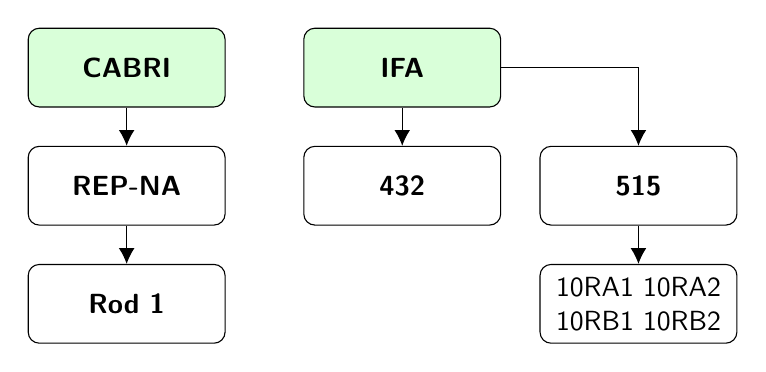
\begin{tikzpicture}[node distance=1.5cm, align=center]

  \node (onIFA)   [box3]                                 {\textbf{IFA}};
  \node (onCABRI) [box3,  left of=onIFA,   xshift=-2.0cm]  {\textbf{CABRI}};
  \node (onREP)   [box0, below of=onCABRI,              ]  {\textbf{REP-NA}};
  \node (onNA)    [box0, below of=onREP,                ]  {\textbf{Rod 1}};
  \node (on515)   [box0, below of=onIFA,   xshift= 3.0cm]  {\textbf{515}};
  \node (on515_)  [box0, below of=on515,   xshift= 0.0cm]  {10RA1 10RA2 \\ 10RB1 10RB2};
  \node (on432)   [box0, below of=onIFA                 ]  {\textbf{432}};

  \draw[->] (onIFA)   -- (on432);
  \draw[->] (onIFA)   -| (on515);
  \draw[->] (on515)   -- (on515_);
  \draw[->] (onCABRI) -- (onREP);
  \draw[->] (onREP)   -- (onNA);
  \end{tikzpicture}
  \end{center} 

\end{frame}
\begin{frame}{}
    \centering
    \Huge{IFA-432 Benchmark}\\
    \large{for FRAPCON cross-verification}
\end{frame}

\begin{frame}{IFA-432 Benchmark Description}
  \footnotesize 

    \begin{block}{\centering{Notes:}}
        \begin{itemize}
            \item Test designed to simulate fuel rods with variations in gap sizes, fuel types and fill gas compositions
            \item The cladding was Zircaloy-2 
            \item Fuel irradiated in Halden BWR (Norway) from 1975 to 1984
            \item The assembly included 6 fuel rods instrumented by 6 vanadium and 1 cobalt neutron detectors,
                  top and bottom centerline termocouples, pressure transducer, elongation sensors and coolant
                  flow meter
            \item The length of fuel rods is 0.635 m
        \end{itemize}
    \end{block}

\end{frame}

\begin{frame}{IFA-432-R3: Fuel burnup and linear power}
  \footnotesize 
  
  \begin{columns}[t]

  \column{.49\textwidth}

  \begin{figure}[h]
    \includegraphics[width=1.\textwidth]{../graphics/IFA-432-r3/average_fuel_burnup}
    \caption{Average fuel burnup}
  \end{figure}  

  \column{.49\textwidth}

  \begin{figure}[h]
    \includegraphics[width=1.\textwidth]{../graphics/IFA-432-r3/average_linear_power}    
    \caption{Average linear power}
  \end{figure}  
  
  \end{columns}

\end{frame}

\begin{frame}{IFA-432-R3 Benchmark (continuous)}
  \footnotesize 
  
  \begin{columns}[t]

  \column{.49\textwidth}

  \begin{figure}[h]
    \includegraphics[width=1.\textwidth]{../graphics/IFA-432-r3/centerline_temperature}
    \caption{Centerline fuel temperature, $C$}
  \end{figure}  

  \column{.49\textwidth}

  \begin{figure}[h]
    \includegraphics[width=1.\textwidth]{../graphics/IFA-432-r3/cladding_average_temperature}    
    \caption{Cladding average temperature, $C$}
  \end{figure}  
  
  \end{columns}

\end{frame}

\begin{frame}{IFA-432-R3 Benchmark (continuous)}
  \footnotesize 
  
  \begin{columns}[t]

  \column{.49\textwidth}

  \begin{figure}[h]
    \includegraphics[width=1.\textwidth]{../graphics/IFA-432-r3/fission_gas_release}
    \caption{Fission gas release}
  \end{figure}  

  \column{.49\textwidth}

  \begin{figure}[h]
    \includegraphics[width=1.\textwidth]{../graphics/IFA-432-r3/oxide_thickness}    
    \caption{Oxide thickness}
  \end{figure}  
  
  \end{columns}

\end{frame}

\begin{frame}{}
    \centering
    \Huge{CABRI REP-NA Benchmark}\\
    \large{for FRAPTRAN cross-verification}
\end{frame}
\begin{frame}{CABRI REP-NA1 Benchmark Description}

    \scriptsize

    \begin{block}{\centering{Notes:}}
        \begin{itemize}
            \item Irradiated 1450 days (60GWd/MTU) in PWR, refabricated and cut rods
            \item Subjected to RIA pulse in the CABRI reactor with 280$C$ flowing sodium
            \item Mesh includes 11 axial nodes, 20 radial nodes in pellet and 5 in cladding
            \item Transient simulation 0...100 ms with the fuel rod power input
        \end{itemize}
    \end{block}


    \begin{figure}[h]
        \includegraphics[width=1.0\textwidth]{figs/cabri_fuel_rod}
    \end{figure}


\end{frame}
\begin{frame}{CABRI REP-NA1: Power and fuel temperature}
  \footnotesize 
  
  \begin{columns}[t]

  \column{.49\textwidth}

  \begin{figure}[h]
    \includegraphics[width=1.\textwidth]{../graphics/rep-na1/average_fuel_rod_power}
    \caption{Average fuel rod power}
  \end{figure}  

  \column{.49\textwidth}

  \begin{figure}[h]
    \includegraphics[width=1.\textwidth]{../graphics/rep-na1/centerline_temperature}
    \caption{Centerline fuel pellet temperature}
  \end{figure}  
  
  \end{columns}

\end{frame}

\begin{frame}{CABRI REP-NA1: Fuel stack and cladding elongation}
  \footnotesize 
  
  \begin{columns}[t]

  \column{.49\textwidth}

  \begin{figure}[h]
    \includegraphics[width=1.\textwidth]{../graphics/rep-na1/cladding_axial_elongation}
    \caption{Cladding axial elongation}
  \end{figure}  

  \column{.49\textwidth}

  \begin{figure}[h]
    \includegraphics[width=1.\textwidth]{../graphics/rep-na1/fuel_stack_elongation}
    \caption{Centerline fuel pellet temperature}
  \end{figure}  
  
  \end{columns}

\end{frame}

\begin{frame}{CABRI REP-NA1: Cladding hoop strain and stress}
  \footnotesize 
  
  \begin{columns}[t]

  \column{.49\textwidth}

  \begin{figure}[h]
    \includegraphics[width=1.\textwidth]{../graphics/rep-na1/cladding_hoop_stress}
    \caption{Cladding hoop stress (MPa)}
  \end{figure}  

  \column{.49\textwidth}

  \begin{figure}[h]
    \includegraphics[width=1.\textwidth]{../graphics/rep-na1/cladding_total_hoop_strain}
    \caption{Cladding total hoop strain ($\%$)}
  \end{figure}  
  
  \end{columns}

\end{frame}

\begin{frame}{CABRI REP-NA1: Gap size and pressure}
  \footnotesize 
  
  \begin{columns}[t]

  \column{.49\textwidth}

  \begin{figure}[h]
    \includegraphics[width=1.\textwidth]{../graphics/rep-na1/gap_pressure}
    \caption{Gap pressure (MPa)}
  \end{figure}  

  \column{.49\textwidth}

  \begin{figure}[h]
    \includegraphics[width=1.\textwidth]{../graphics/rep-na1/structural_radial_gap}
    \caption{Gap size (mm)}
  \end{figure}  
  
  \end{columns}

\end{frame}

\begin{frame}{CABRI REP-NA1: Plenum gas pressure and temperature}
  \footnotesize 

  \begin{columns}[t]

  \column{.49\textwidth}

  \begin{figure}[h]
    \includegraphics[width=1.\textwidth]{../graphics/rep-na1/plenum_gas_pressure}
    \caption{Plenum gas pressure (MPa)}
  \end{figure}

  \column{.49\textwidth}

  \begin{figure}[h]
    \includegraphics[width=1.\textwidth]{../graphics/rep-na1/plenum_gas_temperature}
    \caption{Plenum gas temperature ($\%$)}
  \end{figure}

  \end{columns}

\end{frame}

\begin{frame}{CABRI REP-NA1: Heat transfer coefficient and heat flux}
  \footnotesize 

  \begin{columns}[t]

  \column{.49\textwidth}

  \begin{figure}[h]
    \includegraphics[width=1.\textwidth]{../graphics/rep-na1/surface_heat_flux}
    \caption{Surface heat flux (W/m$^2$)}
  \end{figure}

  \column{.49\textwidth}

  \begin{figure}[h]
    \includegraphics[width=1.\textwidth]{../graphics/rep-na1/heat_transfer_coefficient}
    \caption{Heat transfer coefficient (W/m$^2$K)}
  \end{figure}

  \end{columns}

\end{frame}

\begin{frame}{}
    \centering
    \Huge{Single Rod RIA Simulation}\\
    \large{with the time step control method}
\end{frame}
\begin{frame}{Time Integration Scheme}

    \scriptsize

    \begin{block}{\centering{Features}}
        \begin{itemize}
            \item Double time step method for local error control
            \item Time step rejection option is available
            \item Applicable for any time integration scheme order
        \end{itemize}
    \end{block}

    \begin{figure}[h]
        \includegraphics[width=1.0\textwidth]{figs/time_marching}
    \end{figure}

\end{frame}
\begin{frame}{RIA Pulse: total power and bulk coolant temperature}

    \scriptsize

    \begin{figure}[h]
        \includegraphics[width=0.75\textwidth]{figs/ria-pulse}
    \end{figure}

\end{frame}
\begin{frame}{Numerical integration}

    \scriptsize

    $T_{stop}=200ms$, time iteration tol. $rtol_1=5\cdot10^{-4}$, internal iteration tol. $rtol_2=10^{-7}$

    \begin{block}{\centering{Notes:}}
        \begin{itemize}
            \item Two norms of local error are considered. 
                  $L_{\infty}$ produces more accurate solution while $L_2$ generates
                  less number of rejected time steps
            \item Reference solution was obtained with piece-wise time step history because
                  very small sizes are needed in vicinity of a failure moment.
            \item The watched out parameters are cladding/pellet stress, strain and
                  temperature, gap pressure and heat transfer coefficient
        \end{itemize}
    \end{block}

    \begin{center}{}
        Number of made time steps during simulation\\[1pt]
        \begin{tabular}{c | c | c }
            \hline
            Method              & regular & rejected     \\
            \hline
            Fixed               & 299        & 0   \\
            Simple, $L_2$       & 260        & 64  \\
            Simple, $L_\infty$  & 198        & 97  \\
        \end{tabular}
    \end{center}

\end{frame}
\begin{frame}{Time step history}

    \scriptsize

    \begin{figure}[h]
        \includegraphics[width=0.8\textwidth]{figs/marching}
    \end{figure}

\end{frame}
\begin{frame}{Centerline fuel temperature}

    \scriptsize

    \begin{figure}[h]
        \includegraphics[width=1.0\textwidth]{figs/centerline_temperature,_K}
    \end{figure}

\end{frame}
\begin{frame}{Cladding temperature}

    \scriptsize

    \begin{figure}[h]
        \includegraphics[width=1.0\textwidth]{figs/cladding_inner_temperature,_K}
    \end{figure}

\end{frame}
\begin{frame}{Heat transfer coefficient}

    \scriptsize

    \begin{figure}[h]
        \includegraphics[width=1.0\textwidth]{figs/heat_transfer_coefficient,_W|m^2K}
    \end{figure}

\end{frame}
\begin{frame}{Cladding axial elongation}

    \scriptsize

    \begin{figure}[h]
        \includegraphics[width=1.0\textwidth]{figs/cladding_axial_elongation,_mm}
    \end{figure}

\end{frame}
\begin{frame}{Gap pressure}

    \scriptsize

    \begin{figure}[h]
        \includegraphics[width=1.0\textwidth]{figs/gap_pressure,_MPa}
    \end{figure}

\end{frame}
\begin{frame}{Summary}
    \scriptsize
    \center

    \begin{block}{\textbf{1. Fuel Rod Analysis Program Interface (FRAPI)}}

        \begin{itemize}
            \color{applegreen}
            \item Access to the FRAPCON and FRAPTRAN functions and variables
            \item Step-by-step time integration with the restart capability
            \item Time marching library with time step size control and rejection
            \color{bittersweet}
            \item Large memory costs for the fuel rod state storage
            \item Copy of memory spaces consumes about 40$\%$ of the total computation time
            \item Transient calculation fails when it comes to the coolant boiling
        \end{itemize}

    \end{block}

    \begin{block}{\textbf{2. Cross-verification with the original codes}}

        \begin{itemize}
            \color{applegreen}
            \item Calculated 5 tests of the IFA-432 benchmark and 1 test of the CABRI benchmark
            \item Good coincidence with FRAPCON and FRAPTRAN
            \color{bittersweet}
            \item More benchmark tests must be considered
            \item Fix the difference in the heat transfer coefficient (FRAPTRAN)
        \end{itemize}

    \end{block}

\end{frame}

\end{document}

